% Vodno Ridebook - project report (elaborat).
%
% Build with:  ./scripts/build-elaborat.sh
% Requires XeLaTeX: the architecture diagrams use Unicode box-drawing
% characters, which need a Unicode-aware engine and a monospace font that
% actually carries those glyphs (DejaVu Sans Mono).

\documentclass[10pt,a4paper]{article}

\usepackage{fontspec}
\usepackage[a4paper,top=1.9cm,bottom=1.9cm,left=2.0cm,right=2.0cm]{geometry}
\usepackage{xcolor}
\usepackage{graphicx}
\usepackage{booktabs}
\usepackage{tabularx}
\usepackage{enumitem}
\usepackage{fancyvrb}
\usepackage{titlesec}
\usepackage{caption}
\usepackage{microtype}
\usepackage[hidelinks]{hyperref}

% --- fonts ---------------------------------------------------------------
% The body keeps the default Latin Modern; only the monospace face is
% overridden, because it has to render the box-drawing diagrams.
\setmonofont{DejaVu Sans Mono}[Scale=0.86]

% --- colours -------------------------------------------------------------
\definecolor{accent}{HTML}{B8430A}
\definecolor{rulegrey}{HTML}{C9CFD8}
\definecolor{mutedtext}{HTML}{4A5462}

\hypersetup{
  colorlinks=true,
  linkcolor=accent,
  urlcolor=accent,
  pdftitle={Vodno Ridebook - Project Report},
  pdfauthor={Viktor Najdovski},
}

% --- headings ------------------------------------------------------------
\titleformat{\section}{\Large\bfseries}{\thesection.}{0.5em}{}[\vspace{-0.6em}\textcolor{rulegrey}{\rule{\linewidth}{0.6pt}}]
\titleformat{\subsection}{\normalsize\bfseries}{}{0em}{}
\titlespacing*{\section}{0pt}{1.1em}{0.55em}
\titlespacing*{\subsection}{0pt}{0.75em}{0.28em}

% --- paragraphs (parskip package is not installed here) ------------------
\setlength{\parindent}{0pt}
\setlength{\parskip}{0.42em}

% Let short pages end short rather than stretching the gaps between blocks.
\raggedbottom

% Long \texttt{} runs cannot be hyphenated, so allow slightly looser lines
% rather than letting identifiers spill into the margin.
\setlength{\emergencystretch}{1.6em}
\sloppy

% --- lists ---------------------------------------------------------------
\setlist[itemize]{leftmargin=1.2em,itemsep=0.15em,topsep=0.3em,parsep=0pt}

% --- code and console blocks ---------------------------------------------
\DefineVerbatimEnvironment{code}{Verbatim}
  {frame=single,rulecolor=\color{rulegrey},framesep=6pt,
   fontsize=\scriptsize,samepage=true,xleftmargin=0pt}

% --- tables --------------------------------------------------------------
\renewcommand{\arraystretch}{1.1}
\captionsetup{font=small,labelfont=bf,skip=5pt}

% Shorthand for the many inline identifiers in the text.
\newcommand{\cd}[1]{\texttt{\small #1}}

\begin{document}

% =========================================================================
\begin{center}
  {\LARGE\bfseries Vodno Ridebook\par}
  \vspace{0.35em}
  {\large Project Report\par}
  \vspace{0.9em}
  \begin{tabular}{@{}rl@{}}
    \textbf{Course} & Continuous Integration and Delivery \\
    \textbf{Author} & Viktor Najdovski \\
    \textbf{Repository} & \url{https://github.com/VikiShmiki/vodno-ridebook} \\
  \end{tabular}
\end{center}
\vspace{0.6em}
\textcolor{rulegrey}{\rule{\linewidth}{0.8pt}}

% =========================================================================
\section{Introduction}

\subsection{What Vodno Ridebook is}

Vodno Ridebook is a small web application in the spirit of Waze, but written
for one specific group of users on one specific stretch of road:
motorcyclists riding up to \textbf{Sredno Vodno} in Skopje.

It does two things. Riders can \textbf{report road conditions} --- gravel,
standing water, damaged asphalt, roadworks, heavy traffic, animals, poor
visibility --- each with a severity and a position on the road, and they can
\textbf{log rides}, rating road quality, traffic, cleanliness and enjoyment.
A dashboard combines both into a picture of what the road is like right now.

\subsection{The problem it solves}

A general navigation application answers ``how do I get there''. It does not
answer the question a motorcyclist actually asks before setting off:
\emph{what is the surface like today?} Hazards that a car drives over without
noticing are the ones that matter most on two wheels. A patch of gravel on the
exit of a hairpin, a diesel spill, a pothole in the wheel track --- none of
these appear in a routing app, and all of them change how, or whether, you
ride.

\subsection{Why the Sredno Vodno road}

The road to Sredno Vodno is the default weekend ride for Skopje
motorcyclists: a short, twisty climb out of the city that is busy with riders,
cyclists and hikers. It is a single well-defined route, which keeps the data
model small --- positions can be reported as plain coordinates without any
routing engine --- and it is a road where surface conditions genuinely change
from week to week because of runoff, gravel washed onto the tarmac and
recurring roadworks.

\subsection{Purpose of the project}

The application is deliberately modest. The purpose of the project is the
\textbf{DevOps implementation around it}: taking a realistic three-tier
application and building the complete path from a commit in a Git repository
to a running, self-healing, updatable deployment in Kubernetes. The
application exists to give that pipeline something real to carry:
containerisation, local orchestration with Docker Compose, an automated CI/CD
pipeline in GitHub Actions, publishing to a container registry, and a
Kubernetes deployment with configuration management, persistent storage,
ingress routing, self-healing and zero-downtime rolling updates.

% =========================================================================
\section{Application architecture}

The system is a conventional three-tier application.

\begin{code}
        Browser — React 19 SPA (Vite build, TypeScript)
                          │  REST, relative /api/... paths
                          ▼
   Routing layer:  Vite proxy (dev) · nginx (Compose) · Ingress (K8s)
              │ "/"                        │ "/api"
              ▼                            ▼
   Static bundle (nginx)          FastAPI / uvicorn :8000
                                           │  SQLAlchemy 2.0 · psycopg 3
                                           ▼
                                  PostgreSQL 16
                          motorcycles · rides · road_reports
\end{code}

\subsection{Frontend}

React 19 with Vite and TypeScript, using React Router for four pages ---
Dashboard, Ride log, Road reports and Statistics. There is no state-management
library; a small \cd{useAsync} hook handles loading, error and reload state
for each fetch. Road reports are drawn on an SVG map whose centreline is the
\textbf{real OpenStreetMap geometry} of the climb --- 100 points, simplified to
under one pixel of error, committed to the repository by
\cd{scripts/fetch-road-geometry.py} and projected at a single uniform scale so
the hairpins are undistorted. Reports are snapped to the nearest point on that
line, and a rider files one by clicking the map rather than typing
coordinates. Drawing the road rather than loading map tiles avoids an API key
and a runtime dependency; likewise the icons are inline SVG and the Inter
webfont is served from the image, so the application makes no third-party
request.

\subsection{Backend}

FastAPI with SQLAlchemy 2.0 and Pydantic v2, organised into routers
(\cd{health}, \cd{rides}, \cd{reports}, \cd{motorcycles}, \cd{stats}), ORM
models and Pydantic schemas. Pydantic validates every request: ratings must be
1--5, weather and report categories must be members of the defined
enumerations, and report coordinates must fall inside a bounding box around
the Vodno road. All configuration is read from environment variables through
\cd{pydantic-settings}, so nothing environment-specific is compiled into the
image.

\subsection{Database}

PostgreSQL 16 with three tables --- \cd{motorcycles}, \cd{rides} and
\cd{road\_reports}. \cd{rides.motorcycle\_id} is a nullable foreign key with
\cd{ON DELETE SET NULL}, so a ride remains a valid record after its motorcycle
is removed.

\subsection{Communication between services}

The frontend never uses an absolute API URL. It always requests relative
\cd{/api/...} paths, and whatever sits in front of it decides where they go:

\begin{center}
\begin{tabular}{@{}ll@{}}
\toprule
\textbf{Environment} & \textbf{\cd{/api} is resolved by} \\
\midrule
\cd{npm run dev} & the Vite dev proxy $\rightarrow$ \cd{localhost:8000} \\
Docker Compose   & nginx in the frontend container $\rightarrow$ \cd{backend:8000} \\
Kubernetes       & the Ingress $\rightarrow$ the backend Service \\
\bottomrule
\end{tabular}
\end{center}

This is the single most useful decision in the project: \textbf{the same
frontend image runs unchanged in every environment}, which is what makes ``the
artifact tested in CI is the artifact deployed to production'' true rather
than aspirational.

\subsection{API surface}

Twelve REST endpoints are served under \cd{/api}, with interactive
documentation at \cd{/api/docs}: full CRUD for \cd{rides} and \cd{reports},
list/create for \cd{motorcycles}, an aggregate \cd{stats} endpoint and
\cd{health}. The complete table is in the README.

\cd{GET /api/health} runs \cd{SELECT 1} against the database and returns
\cd{503} when that fails. This matters for the Kubernetes section: a pod that
has lost its database is taken out of the Service endpoints instead of
returning errors.

% =========================================================================
\section{Dockerization}

Both services are containerised separately with multi-stage builds.

\subsection{Backend Dockerfile}

Stage one, on \cd{python:3.12-slim}, creates a virtualenv at \cd{/opt/venv}
and installs the pinned requirements. Stage two starts from the same slim base,
copies only the finished virtualenv and the \cd{app} package, and never sees
pip's caches or build tooling. It applies outstanding OS security patches,
creates a dedicated user and ends with \cd{USER vodno} (uid 1001), so no
application code runs as root. A \cd{HEALTHCHECK} calls \cd{/api/health} using
the standard library, avoiding an extra \cd{curl} dependency.

\subsection{Frontend Dockerfile}

Stage one, on \cd{node:24-alpine}, copies the lockfile and runs \cd{npm ci}
before the source, so the dependency layer is reused whenever only application
code changes, then runs \cd{npm run build}. Stage two is
\cd{nginxinc/nginx-unprivileged:1.27-alpine}, which listens on 8080 as uid 101
without root and receives only the compiled \cd{dist} directory plus an nginx
configuration template.

\subsection{Resulting images}

\begin{center}
\begin{tabular}{@{}lll@{}}
\toprule
\textbf{Image} & \textbf{Size} & \textbf{Runs as} \\
\midrule
\cd{vodno-frontend} & 74.4 MB & \cd{uid=101(nginx)} \\
\cd{vodno-backend}  & 311 MB  & \cd{uid=1001(vodno)} \\
\bottomrule
\end{tabular}
\end{center}

Both were verified with \cd{docker compose exec <service> id} in the running
containers.

\subsection{Important configuration decisions}

\begin{itemize}
  \item \textbf{Nothing is hardcoded.} The backend reads database host, port,
        name, credentials, CORS origins and log level from the environment.
        The frontend's nginx configuration is a template with a
        \cd{\$\{BACKEND\_URL\}} placeholder that the nginx entrypoint renders
        with \cd{envsubst} at container start --- so the proxy target can
        change without rebuilding the image.
  \item \textbf{\cd{.dockerignore} in both contexts} keeps \cd{node\_modules},
        \cd{.venv}, test directories, caches and any \cd{.env} file out of the
        build context. Excluding \cd{.env} is a security measure as much as a
        size one.
  \item \textbf{nginx serves the SPA correctly}: \cd{try\_files} falls back to
        \cd{index.html} so client-side routes work on a hard refresh,
        \cd{index.html} is sent with \cd{Cache-Control: no-store} so a rolling
        update is picked up on reload, while hashed assets under \cd{/assets/}
        are marked immutable for a year.
\end{itemize}

% =========================================================================
\section{Docker Compose}

\begin{code}
cp .env.example .env
docker compose up --build
\end{code}

The application is then available at \url{http://localhost:8080}.

\subsection{The three services}

\begin{center}
\begin{tabular}{@{}llll@{}}
\toprule
\textbf{Service} & \textbf{Image} & \textbf{Port} & \textbf{Role} \\
\midrule
\cd{postgres} & \cd{postgres:16-alpine}   & 5432 internal & Database \\
\cd{backend}  & built from \cd{./backend} & 8000          & FastAPI API \\
\cd{frontend} & built from \cd{./frontend}& 8080 $\rightarrow$ 8080 & Static bundle + \cd{/api} proxy \\
\bottomrule
\end{tabular}
\end{center}

\subsection{Networking}

All three join a user-defined bridge network, \cd{vodno-network}, and address
each other by service name --- the backend connects to \cd{postgres:5432}, and
nginx proxies to \cd{backend:8000}. PostgreSQL deliberately publishes
\textbf{no} host port; it is reachable only from inside the network.

\subsection{Environment variables}

Every value comes from \cd{.env}, which is created from the committed
\cd{.env.example} and is itself git-ignored. Compose substitutes defaults with
the \cd{\$\{VAR:-default\}} syntax, so the stack still starts if a variable is
missing.

\subsection{PostgreSQL persistence}

The database directory is a named volume, \cd{vodno\_postgres\_data}, with
\cd{PGDATA} pointing one level below the mount point. Data therefore survives
\cd{docker compose down}; only \cd{docker compose down -v} removes it.
Verified:

\begin{code}
$ docker compose down && docker compose up -d
$ curl -s http://localhost:8080/api/rides | python3 -c "import sys,json;print(len(json.load(sys.stdin)))"
7
\end{code}

\subsection{Health checks and dependencies}

Each service defines a health check --- \cd{pg\_isready} for PostgreSQL, an
HTTP call to \cd{/api/health} for the backend, and \cd{/healthz} for the
frontend --- and \cd{depends\_on} uses \cd{condition: service\_healthy}.
Compose therefore starts them in strict order: postgres becomes healthy, then
the backend, then the frontend.

\begin{code}
SERVICE    STATE     STATUS                   PORTS
backend    running   Up 2 minutes (healthy)   0.0.0.0:8000->8000/tcp
frontend   running   Up 8 seconds (healthy)   0.0.0.0:8081->8080/tcp
postgres   running   Up 2 minutes (healthy)   5432/tcp
\end{code}

% =========================================================================
\section{CI/CD pipeline}

Two workflows, in \cd{.github/workflows/}.

\subsection{\cd{ci.yml} --- pull requests and feature branches}

\begin{code}
checkout
  ├─ frontend  → npm ci → oxlint → tsc -b → Vitest → vite build → upload dist
  ├─ backend   → pip install → ruff check → ruff format --check
  │               → pytest against a PostgreSQL 16 service container
  │               → assert the OpenAPI schema exposes the required routes
  ├─ docker-build       → Buildx builds both images, then Trivy scans them
  ├─ elaborat           → compile this report with XeLaTeX, strictly
  └─ compose-smoke-test → docker compose up --build -d, then curl
                          /healthz, /api/health, /api/stats, /api/reports
\end{code}

Three details are worth calling out. First, the backend suite runs against a
real \textbf{PostgreSQL 16 service container}, the same major version used in
Compose and Kubernetes, rather than against a substitute database. Second, the
\cd{compose-smoke-test} job starts the entire stack and exercises it over
HTTP, so a change that passes the unit tests but breaks the container wiring
--- a wrong proxy target, a missing environment variable --- is caught before
merge. Third, this report is itself built by the pipeline: the \cd{elaborat}
job compiles it with XeLaTeX and fails on an overfull box, a glyph the fonts
cannot render, or a page count outside the required range, then publishes the
PDF as a build artifact. Nothing is published from a pull request.

\subsection{\cd{cd.yml} --- pushes to \cd{main}}

\begin{code}
git push to main
      ↓
CI gate  (ci.yml re-used via workflow_call — byte-identical checks)
      ↓
build both images with Buildx (GitHub Actions layer cache)
      ↓
push to ghcr.io, tagged:  latest · <short-sha> · <full-sha>
      ↓
deploy on a self-hosted runner sitting next to the cluster
  kubectl apply → kubectl set image → rollout status → Ingress smoke test
  └─ on failure: roll back to the previously running images
\end{code}

Re-using \cd{ci.yml} through \cd{workflow\_call} rather than copying the steps
means \cd{main} can never be published under weaker checks than a pull
request.

\subsection{Image tagging}

\begin{code}
ghcr.io/vikishmiki/vodno-backend:latest · :<short-sha> · :<full-sha>
ghcr.io/vikishmiki/vodno-frontend:latest · :<short-sha> · :<full-sha>
\end{code}

\cd{latest} is the readable tag used by the manifests; the commit SHA is the
immutable one used by the deployment step, so any running pod can be traced
back to the exact commit it was built from. OCI labels record the source
repository and revision inside the image itself.

\subsection{Supply chain security}

Every image is scanned with Trivy before it can be published. The build
\textbf{fails} on a HIGH or CRITICAL vulnerability that has a fix available;
unfixed CVEs are reported to the repository's Security tab as SARIF rather
than blocking, because the project cannot act on them until upstream patches.
A CycloneDX SBOM is published alongside each image, which answers ``what is
actually in this container'' in a way a CVE list alone does not.

Introducing the scan was not a formality. It found \cd{starlette 0.41.3}
carrying three HIGH CVEs, pinned transitively by the FastAPI version in use,
and both base images shipping unpatched OS packages. Upgrading FastAPI and
adding a security-update layer to each runtime stage took the count of
fixable HIGH/CRITICAL findings from 87 in the backend image and 35 in the
frontend to \textbf{zero in both}, so the gate starts from a clean state.

\subsection{Secrets}

No credential appears in any file in the repository. \cd{GITHUB\_TOKEN},
provided automatically by GitHub Actions, is the only one needed: it
authenticates the push to GHCR. The deployment step needs no secret at all,
because it runs on a machine that already has cluster access.

\subsection{Deployment and branch protection}

A GitHub-hosted runner cannot reach a kind cluster running on a laptop, so
the \cd{deploy} job runs on a \textbf{self-hosted runner} installed next to
the cluster. It applies the manifests, rolls both Deployments to the
commit-SHA tag, waits for the rollouts, and then smoke-tests the application
through the Ingress --- a green rollout only proves the pods started, not
that they serve. If any step fails, the previously running images are
restored automatically.

Only this job is self-hosted, and it triggers solely on a push to \cd{main},
never on a pull request, so code from a fork cannot execute on the machine.
Every CI job stays on a GitHub-hosted runner.

\cd{main} is a protected branch: no direct pushes, no force pushes, no
deletion, and all six CI checks must pass before a pull request can merge.
The rules are enforced for administrators too, which is what makes the
pipeline a gate rather than a suggestion.

\subsection{CD mechanism}

The chosen approach is GitHub Actions running \cd{kubectl} directly. It is a
single readable file, it needs nothing installed in the cluster, and the whole
mechanism can be explained in one slide. Argo CD was considered and rejected
as more infrastructure than this project can justify; the trade-off is noted
in \cd{docs/architecture.md}.

The workflows are linted with \cd{actionlint}, which reports no findings.

% =========================================================================
\section{Kubernetes architecture}

Everything runs in a dedicated namespace, \textbf{\cd{vodno-ridebook}}.

\begin{code}
                    Internet / laptop  →  http://vodno.local
                                  │
                      ingress-nginx  ·  Ingress vodno-ingress
                     "/" │                          │ "/api"
                         ▼                          ▼
              Service frontend :80         Service backend :8000
                 (ClusterIP)                    (ClusterIP)
                    │      │                     │      │
              ┌─────┘      └─────┐         ┌─────┘      └─────┐
           frontend pod    frontend pod  backend pod    backend pod
           nginx :8080     nginx :8080     :8000          :8000
           probe /healthz                  probe /api/health
                                                 │
                                    Service postgres (headless)
                                                 │
                                     postgres-0  (StatefulSet)
                                                 │
                                  PVC data-postgres-0 · 1Gi · RWO

   ConfigMap vodno-config → backend, frontend
   Secret    vodno-secret → backend, postgres
   Namespace vodno-ridebook contains everything above
\end{code}

\subsection{Namespace}

\cd{vodno-ridebook} isolates the application: the whole system can be
inspected with \cd{kubectl get all -n vodno-ridebook} and removed with one
namespace deletion.

\subsection{Deployments and replicas}

The backend and frontend each run \textbf{two replicas} with
\cd{podAntiAffinity} preferring different nodes. Both use a
\cd{RollingUpdate} strategy with \cd{maxUnavailable: 0} and \cd{maxSurge: 1},
and both set CPU and memory requests and limits.

\subsection{Services}

\cd{frontend} (ClusterIP :80) and \cd{backend} (ClusterIP :8000) are ordinary
ClusterIP Services. \cd{postgres} is \textbf{headless}
(\cd{clusterIP: None}), which is the right pairing for a StatefulSet: it gives
the pod the stable DNS name
\cd{postgres-0.postgres.vodno-ridebook.svc.cluster.local}, and the backend
simply connects to \cd{postgres}.

\subsection{Ingress}

One \cd{Ingress} object, one hostname. \cd{ingress-nginx} matches Prefix rules
longest-first, so \cd{/api} reaches the backend and everything else falls
through to the frontend --- the entire application is served from
\cd{http://vodno.local}.

\subsection{ConfigMap and Secret}

\cd{vodno-config} holds eight non-sensitive settings: application environment,
log level, database host, port and name, CORS origins, the seed flag and the
frontend's backend URL. \cd{vodno-secret} holds \cd{POSTGRES\_USER} and
\cd{POSTGRES\_PASSWORD}. The backend consumes both with \cd{envFrom};
PostgreSQL uses \cd{secretKeyRef} and \cd{configMapKeyRef}.

\textbf{No real credential is committed.} The committed template
\cd{k8s/examples/secret.example.yaml} carries nothing but the placeholder
value, and it lives in a subdirectory precisely because
\cd{kubectl apply -f k8s/} does not recurse --- it cannot be applied by
accident. The deployment script generates the real Secret imperatively:

\begin{code}
kubectl -n vodno-ridebook create secret generic vodno-secret \
  --from-literal=POSTGRES_USER=vodno \
  --from-literal=POSTGRES_PASSWORD="$(openssl rand -base64 24)"
\end{code}

\subsection{PostgreSQL StatefulSet and PersistentVolumeClaim}

PostgreSQL runs as a StatefulSet with one replica and a
\cd{volumeClaimTemplates} entry requesting 1\,Gi \cd{ReadWriteOnce} storage.
This produces the claim \cd{data-postgres-0}, which is re-attached to the pod
on every restart. The pod runs as uid 999 with \cd{fsGroup: 999} so the
mounted volume is writable.

\subsection{Health probes}

\begin{center}
\begin{tabular}{@{}llll@{}}
\toprule
\textbf{Workload} & \textbf{Startup} & \textbf{Readiness} & \textbf{Liveness} \\
\midrule
\cd{backend}  & \cd{/api/health}, up to 90\,s & \cd{/api/health}, 10\,s & \cd{/api/health}, 20\,s \\
\cd{frontend} & ---                           & \cd{/healthz}, 10\,s    & \cd{/healthz}, 20\,s \\
\cd{postgres} & ---                           & \cd{pg\_isready}, 5\,s  & \cd{pg\_isready}, 15\,s \\
\bottomrule
\end{tabular}
\end{center}

The backend's startup probe gives it time to wait for PostgreSQL on a cold
start without the liveness probe killing it. The frontend probes
\cd{/healthz}, which nginx answers itself --- a backend outage must not
restart the web tier.

\subsection{Security context}

Both application pods run with \cd{runAsNonRoot},
\cd{readOnlyRootFilesystem: true}, \cd{allowPrivilegeEscalation: false}, all
capabilities dropped and the \cd{RuntimeDefault} seccomp profile; the few
writable paths each service needs are \cd{emptyDir} volumes.

% =========================================================================
\section{Kubernetes demonstrations}

All output below is copied from real runs on a three-node kind cluster
(Kubernetes v1.34.0) with \cd{ingress-nginx}. The full guide is in
\cd{docs/demos.md}.

\subsection{Cluster state}

\begin{code}
$ kubectl get pods -n vodno-ridebook -o wide
NAME                        READY   STATUS    RESTARTS   NODE
backend-b55bd665b-2qcdw     1/1     Running   0          vodno-worker
backend-b55bd665b-5qbgr     1/1     Running   0          vodno-worker2
frontend-788ff4c77c-tqhcl   1/1     Running   0          vodno-worker2
frontend-788ff4c77c-vjqmh   1/1     Running   0          vodno-worker
postgres-0                  1/1     Running   0          vodno-worker2

$ kubectl get services -n vodno-ridebook
NAME       TYPE        CLUSTER-IP      PORT(S)
backend    ClusterIP   10.96.186.215   8000/TCP
frontend   ClusterIP   10.96.127.44    80/TCP
postgres   ClusterIP   None            5432/TCP

$ kubectl get ingress -n vodno-ridebook
NAME            CLASS   HOSTS         PORTS   AGE
vodno-ingress   nginx   vodno.local   80      31s
\end{code}

The anti-affinity rule placed the two backend replicas on different worker
nodes, which is what makes the self-healing demonstration meaningful.

\subsection{Access through the Ingress}

\begin{code}
$ curl -s http://vodno.local/api/health
{"status":"healthy","database":"connected","version":"1.0.0","environment":"production"}

$ curl -o /dev/null -s -w "%{http_code}\n" http://vodno.local/        # 200
$ curl -o /dev/null -s -w "%{http_code}\n" http://vodno.local/stats   # 200
\end{code}

The last request is a client-side route: nginx falls back to \cd{index.html}
and React Router renders the Statistics page.

\begin{figure}[htbp]
  \centering
  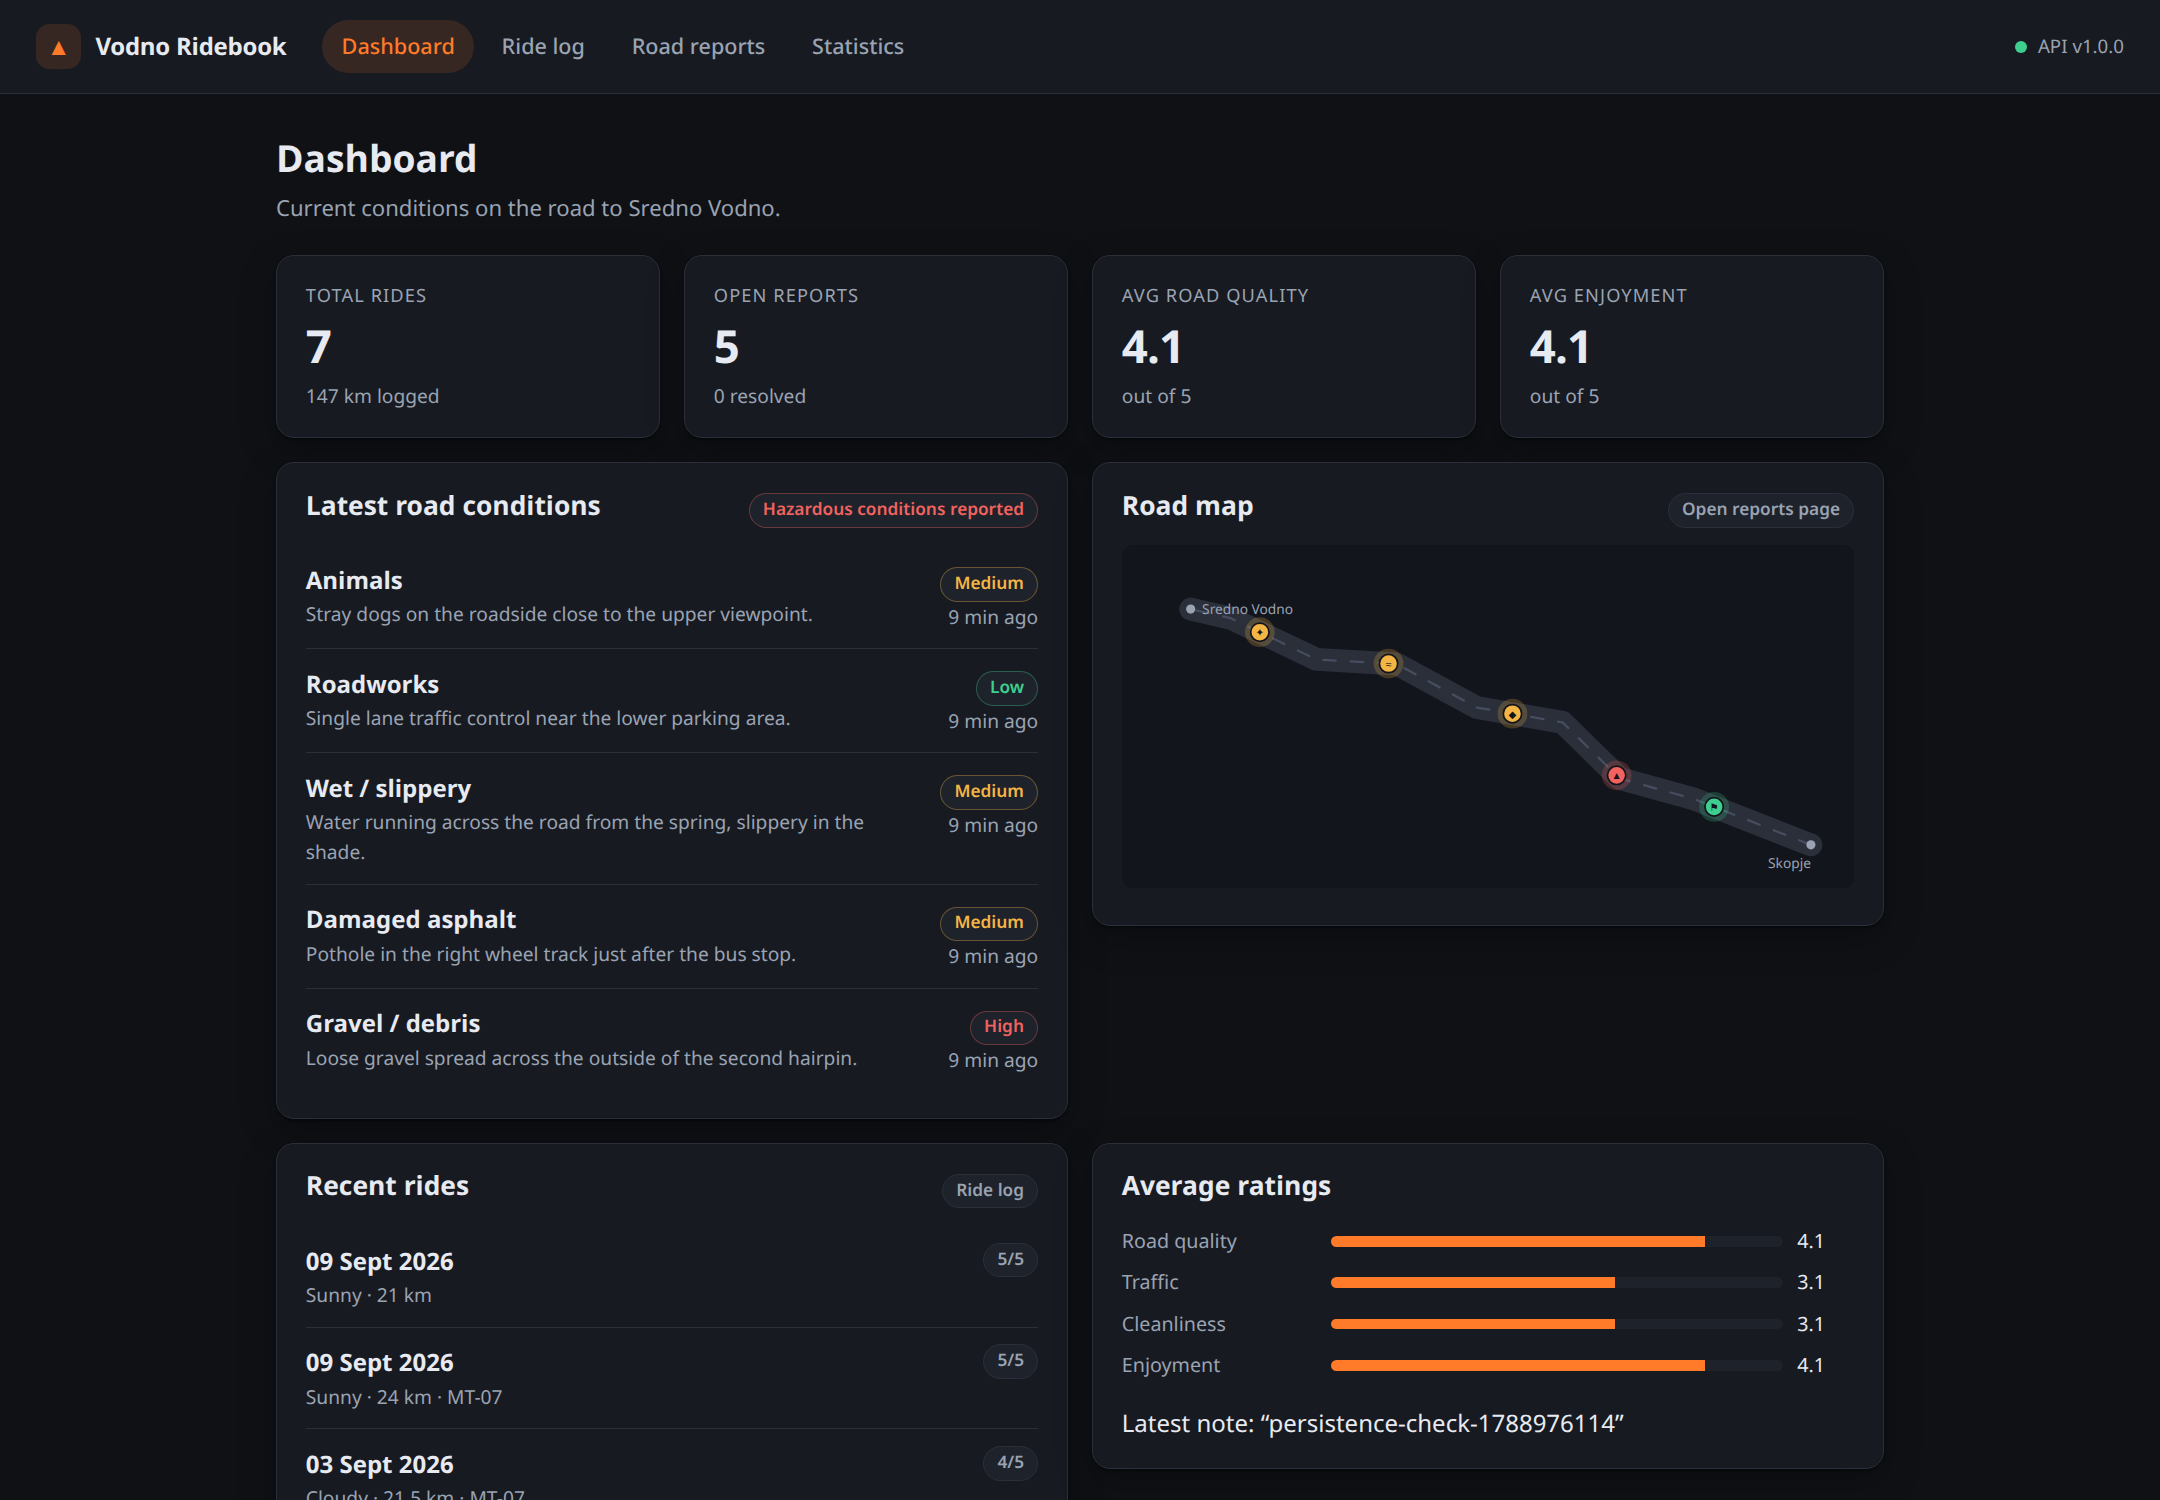
\includegraphics[width=0.72\linewidth]{images/dashboard.png}
  \caption{The dashboard at \cd{http://vodno.local}, served by the frontend
  pods with data fetched from the backend pods --- both reached through the
  single Ingress.}
\end{figure}

\subsection{ConfigMap and Secret reaching the container}

\begin{code}
$ kubectl exec -n vodno-ridebook backend-5947bbb96c-bbbf7 -- \
    printenv APP_ENV POSTGRES_HOST POSTGRES_DB CORS_ORIGINS
production
postgres
vodno
http://vodno.local
\end{code}

The Secret arrives the same way, and the password is the one generated at
deployment time rather than anything taken from the repository:

\begin{code}
$ kubectl get secret vodno-secret -n vodno-ridebook \
    -o jsonpath="{.data.POSTGRES_USER}" | base64 -d
vodno
\end{code}

\subsection{Self-healing}

\cd{./scripts/demo-self-healing.sh} polls \cd{/api/health} twice a second
while one backend pod is deleted.

\begin{code}
==> Polling the API while 'backend-b55bd665b-2qcdw' is deleted
.pod "backend-b55bd665b-2qcdw" deleted from vodno-ridebook namespace
...........................................................

==> Backend pods after (a replacement is created automatically)
NAME                      READY   STATUS    RESTARTS   AGE   NODE
backend-b55bd665b-5qbgr   1/1     Running   0          81s   vodno-worker2
backend-b55bd665b-xhcwh   1/1     Running   0          31s   vodno-worker

Legend: '.' = request served, 'X' = request failed
\end{code}

\textbf{60 of 60 requests were served; none failed.} The ReplicaSet scheduled
\cd{backend-b55bd665b-xhcwh} as a replacement while the surviving replica
continued to answer.

\subsection{Persistent database storage}

\cd{./scripts/demo-persistence.sh} writes a uniquely tagged ride, deletes
\cd{postgres-0}, and checks the data afterwards.

\begin{code}
==> Writing a ride tagged 'persistence-check-1788976855'
    total rides before: 7

NAME              STATUS   VOLUME                       CAPACITY   ACCESS MODES
data-postgres-0   Bound    pvc-67cdb7fa-01bc-47b1-…     1Gi        RWO

==> Deleting the PostgreSQL pod
pod "postgres-0" deleted from vodno-ridebook namespace
pod/postgres-0 condition met

    total rides after : 7
    marker rides found: 1
PASS: the data survived the pod deletion
\end{code}

The recreated pod kept the name \cd{postgres-0} and re-bound the same claim. A
Deployment would have produced a pod with a new random name and, without a
claim template, an empty database.

\subsection{Rolling update}

\cd{./scripts/demo-rolling-update.sh v2} builds a new tag and rolls it out
while polling the API.

\begin{code}
==> Image currently running:  ghcr.io/vikishmiki/vodno-backend:latest

==> Rolling out while polling the API
.deployment.apps/backend image updated
Waiting for rollout: 1 out of 2 new replicas have been updated...
..................Waiting for rollout: 1 old replica is pending termination...
...................deployment "backend" successfully rolled out
..........................................

==> Image now running:  ghcr.io/vikishmiki/vodno-backend:v2
\end{code}

\textbf{80 of 80 requests were served with zero failures.}

This result was not free. The first measured rollout recorded one failed
request: endpoint removal and \cd{SIGTERM} reach a terminating pod
concurrently, so for a moment the Ingress could still route to a pod that had
started shutting down. A five-second \cd{preStop} hook, which removes the pod
from the load balancers before uvicorn shuts down, brought the failure count
to zero --- a good illustration of why ``zero downtime'' has to be measured,
not assumed.

% =========================================================================
\section{Results and conclusion}

\subsection{What was implemented}

A complete, working path from source code to a running Kubernetes deployment:

\begin{itemize}
  \item A three-tier application with 47 automated tests (22 backend, 25
        frontend), clean linting on both sides and a database-aware health
        endpoint.
  \item Multi-stage Docker images for both services (74\,MB and 311\,MB),
        non-root with read-only root filesystems.
  \item A Docker Compose stack with health checks, ordered startup, a private
        network and a persistent named volume.
  \item A CI pipeline: linting, type checking, tests against a real
        PostgreSQL service container, an OpenAPI contract assertion, image
        builds, Trivy vulnerability scanning with SBOM publication, a full
        Compose smoke test and a strict build of this report --- all six
        enforced as required checks on a protected \cd{main}.
  \item A CD pipeline re-using that gate, publishing to GHCR under
        \cd{latest} and commit-SHA tags, then deploying to the cluster from a
        self-hosted runner with a post-deploy smoke test and automatic
        rollback.
  \item Kubernetes manifests: dedicated namespace, ConfigMap, Secret (safe
        committed template), PostgreSQL StatefulSet with a
        PersistentVolumeClaim, two-replica Deployments with probes, limits,
        anti-affinity and a PodDisruptionBudget, and an Ingress serving
        everything on one hostname.
  \item Scripted demonstrations of self-healing, persistence and
        zero-downtime rolling updates, all verified on a real three-node
        cluster.
\end{itemize}

\subsection{Technologies used}

\begin{center}
\begin{tabular}{@{}ll@{}}
\toprule
\textbf{Area} & \textbf{Technology} \\
\midrule
Version control & Git, GitHub \\
Frontend        & React 19, Vite 8, TypeScript, React Router, oxlint, Vitest \\
Backend         & Python 3.12, FastAPI, SQLAlchemy 2, Pydantic v2, ruff, pytest \\
Database        & PostgreSQL 16 \\
Containers      & Docker, multi-stage builds, Docker Compose \\
CI/CD           & GitHub Actions, Buildx, actionlint, Dependabot \\
Registry        & GitHub Container Registry (GHCR) \\
Orchestration   & Kubernetes 1.34, kind, ingress-nginx, kubectl \\
\bottomrule
\end{tabular}
\end{center}

\subsection{What was learned}

Three things stand out.

\textbf{Running the demonstrations found real bugs.} Deploying two backend
replicas exposed a startup race in which both seeded the database, producing
twelve rides instead of six --- something a single replica or Docker Compose
could never have revealed. The fix, running schema creation and seeding inside
a PostgreSQL advisory lock, applies to any multi-replica service with startup
work.

\textbf{``Zero downtime'' is a measurement, not a configuration flag.} Setting
\cd{maxUnavailable: 0} and adding readiness probes felt like enough, and the
rollout still dropped a request. Only polling the API through the rollout
revealed it, and only then did the missing piece --- a \cd{preStop} drain hook
--- become obvious.

\textbf{A pipeline that cannot deploy is only half a pipeline.} For most of
this project the \cd{deploy} job was skipped on every single run, because no
cluster was reachable from a hosted runner. The workflow looked complete and
proved nothing. Installing a self-hosted runner beside the cluster was what
turned continuous integration into continuous delivery, and adding a
post-deploy smoke test with automatic rollback is what made that delivery
trustworthy rather than merely automatic.

\textbf{Small architectural decisions pay off across the pipeline.} Choosing
relative \cd{/api} paths instead of a build-time API URL meant one frontend
image for every environment. That one decision is what makes the CI smoke test
meaningful: the container tested in the pipeline is byte-identical to the one
that runs in Kubernetes.

\subsection{Possible future improvements}

\begin{itemize}
  \item \textbf{Authentication} --- JWT, with the signing key added to the
        existing Secret.
  \item \textbf{Alembic migrations} in an init container, replacing
        \cd{create\_all} once the schema starts to evolve.
  \item \textbf{Observability} --- a Prometheus metrics endpoint, a Grafana
        dashboard and structured JSON logs.
  \item \textbf{Argo CD} --- moving to GitOps would remove the ordering
        constraint between \cd{kubectl apply} and \cd{kubectl set image}.
  \item \textbf{A highly available database}, for example via the CloudNativePG
        operator.
  \item \textbf{GPS capture on a phone}, so a report can be filed at the
        roadside without finding the spot on the map first.
\end{itemize}

\subsection{Conclusion}

The project set out to demonstrate a complete continuous integration and
delivery workflow rather than a large application, and the small size of Vodno
Ridebook turned out to be the right choice: it left room to get the pipeline
right, to measure what it claimed, and to fix every defect that measurement
uncovered --- a seeding race, a dropped request during rollout, and a set of
vulnerable dependencies. The result is a system that can be built, tested,
scanned, published, deployed, verified and rolled back without a manual step
outside \cd{git push}.

\end{document}
